\documentclass[12pt, a4paper]{article}
\usepackage[utf8]{inputenc}
\usepackage[sorting=none]{biblatex}
\usepackage{setspace}
\usepackage{comment}
\usepackage{verbatim}
\usepackage{subcaption, titlesec, fullpage, listings, float, amssymb, amsmath, amsfonts, graphicx, indentfirst, pdfpages}
\usepackage[space]{grffile}
\usepackage{amsmath} 
\usepackage{graphicx} %package to manage images
\graphicspath{ {./plots/} }
\usepackage[rightcaption]{sidecap}
\usepackage{wrapfig}
\usepackage[framed,numbered,autolinebreaks,useliterate]{mcode}
\usepackage{tocbibind}


% custom functions
\titleformat{\section}{\normalfont\Large\bfseries}{\thesection}{1em}{}[{\titlerule[0.8pt]}]

% config settings
% \addbibresource{references.bib}
\captionsetup{font=footnotesize}
\setlength{\parskip}{1em}

\bibliography{references}

\doublespacing
\begin{document}
{\begin{titlepage}
    \begin{center}
        \vspace*{3cm}
        \Huge\textbf{Amath 383 Final Project}
        
        \Huge\textbf{Modeling the Outbreak of COVID-19}
        
        \vspace{2cm}
        
        \Large March 12, 2020 \\
        \Large Author: Tahmin Raj Talukder
        
    \end{center}


\end{titlepage}}

\tableofcontents


\newpage
\section{Abstract}

In this paper, we investigate various techniques and models for viral epidemics in regards to the recent outbreak of COVID-19 caused by coronavirus. We will utilize SIR and SEIR models using parameters based on statistical data of the outbreak to understand the potential outcomes of the disease and better evaluate the risk of epidemic. We found that we would expect epidemic conditions under practical circumstances. We also examine the potential benefits of having a vaccine, and the critical level of vaccination needed in the population in order to prevent an epidemic scenario. Overall, we expect the situation to worsen in the United States as measures taken to combat the spread are insufficient based on our findings.

\section{Introduction}

In a grand sense, infectious disease has been one of mankind's greatest enemies throughout our history on earth. Notoriously, we have overcome outbreaks in antiquity such as the Black Plague, which has been estimated at killing at least one-third of the population of Europe. In more recent history, there have been outbreaks like the Spanish Influenza Epidemic in 1918. Outbreaks such as these are responsible for millions of deaths and have presented a great challenge for the human race to overcome. Recent advances in medicine and vaccination have made deadly disease outbreaks more infrequent in the modern world, but there is plenty of evidence that they still present a challenge to our society and collective health. These have included strains of viruses like the Avian flu, Swine flu, MERS, SARS, and more deadly diseases like Ebola. These can present widespread and potentially catastrophic outcomes, which have been readily apparent in popular culture. 

The first case of COVID-19 was reported in Wuhan, China, and has since spread across the country and across international borders \cite{center}. The World Health Organization (WHO) has now confirmed that there are over 85,000 cases of COVID-19 across the world as of writing this paper \cite{center}. The disease has continued to spread at an alarming rate, with new cases being reported in over 50 countries worldwide. The severity of the epidemic is still to be determined, but there is little doubt of the potential that this has to cause catastrophic damage to populations across the globe. 

According to the CDC, the virus that causes COVID-19 mainly spreads by person-to-person through close contact and respiratory droplets when a person sneezes or coughs \cite{center}. A person may get infected by touching an infected surface with the virus \cite{center}. Symptoms of COVID-19 appear anywhere from 2 to 14 days of infection and include fever, cough, or shortness of breath \cite{center}. Though these effects of COVID-19 are local from person to person, there is much more at stake for countries in terms of political power and economic stability. Thus, it is imperative that mathematical models be developed to better estimate risks and be more prepared for the dynamic progression of the disease.

Modeling of epidemics has been a practice in use for quite some time. In 1927, Kermack and McKendrick developed a model for investigating different populations overtime of an epidemic \cite{kermack}. Their model would give birth to the commonly used SIR model. Simple models such as this can be extremely useful for understanding the potential outbreaks of disease. If we can use these models to predict what may happen within the population in regards to a disease, we can better understand what needs to be done in order to deal with that disease. As we have made clear, these situations should not be taken lightly, as diseases such as this are responsible for millions of deaths. If we can use tools to better comprehend the trajectory of such things, that power should not be taken for granted.

Along with the SIR model, there are plenty of variations to these deterministic models. Deterministic models attempt to assign subgroups of the population to different compartments, such as a susceptible population in the SIR model \cite{sir}. Other models include the SI model, SIRS model, SEIR model, and SEIRS model. These all use variations in the different subgroups of the population and also use different formulations for the rate of change of those subgroups. They can factor in different changes in the population as well, such as the natural birth and death rates. These models utilize the fact that the entire population moves between these compartments. Due to this, we can investigate how these different compartments will change over time. Using real data to see the rate of infection and recovery allows us to predict how the disease will move throughout the entire population in the region. The system of differential equations that we will use employs these known facts.

 We will restrict our analysis first to the population of just the people of the Hubei Province in China. We believe it is important to understand the localized effects of an outbreak to understand how the disease will work. Additionally, attempting to model travel across international borders with active screening and quarantining presented too great of a challenge for the scope of our paper. In a recently published paper, researchers used an extended version of the SEIR model to simulate and predict the outcomes of the spread of the virus in Wuhan and other parts of China \cite{control}. The model considers many factors of the disease. For example, asymptomatic and symptomatic infected people were separated to distinguish different detection and recovery rates. Emigration rates, detection rates, and quarantine rates of both infected and susceptible people were also taken into account in the model, having them vary over time. What we can learn from this paper is that there are more variations that can be continually added to the standard SEIR model in order to create a more realistic picture of real life scenarios, making it much more detailed and complex than the basic model.

There are more complex techniques of disease modeling, known as stochastic models. These attempt to utilize random variables to simulate fluctuations in historical data. However, they are much more challenging to compute, and therefore we will only be investigating the compartmental models that we have already described above. We believe that these models are sufficient to gain an understanding of the disease and its spread and it is not needed to create a more complex model for the scope of our investigation. However, a situation with more serious implications, a governments decisions on travel for example, would require a more rigorous and realistic model such as this.

In this paper, we will use these models in an attempt to discern information about COVID-19. We are in a unique position to do this because of the immediateness of our results. We could utilize these analytical tools at any time, but this opportunity gives us the chance to see how our findings hold up in real-time. While our models might be relatively simple, the basic structure and motivation behind our methods is something that any major government or medical body is doing. We believe that our motivations in writing this paper are clear and transparent and that they are not overlooked by the general population.


\section{Models}
    
    \subsection{SIR Model}
    We will first do an analysis of a standard SIR model. This model uses the three compartments in the name of the model, the susceptible, infectious, and recovered subgroups. 
    
    \subsubsection{Formulation}
    We will formulate the system of differential equations below. The variables and parameters needed to explain these equations are listed below:
    
        \begin{align*}
        S &= \text{ number of susceptible individuals}\\
        I &= \text{ number of infected individuals}\\
        R &= \text{ number of recovered individuals}\\
        N &= \text{ total population}\\
        \beta &= \text{rate of infection}\\
        \gamma &= \text{rate of recovery}\\
        \end{align*}
        The system of differential equations thus becomes as follows:
        \begin{align*}
            \frac{dS}{dt} &= -\frac{\beta SI}{N} \\
            \frac{dI}{dt} &= \frac{\beta SI}{N} - \gamma I \\
            \frac{dR}{dt} &= \gamma I.
        \end{align*}
        And we have $S + I + R = N$.
        Thus, the total population is comprised of the total sum of each of the compartments of the population.
        
        We can see that the susceptible population changes because of both the amount of the susceptible population and the amount of the infected population. If there are more susceptible individuals, more people will become infected. If there are more infected individuals, they can spread the disease to more people. We can see that the infected equation has this term as well, indicating that people are moving from the susceptible population to the infected population. The infected equation also has a term that only has the infected population. Recovering from the infection is only determined by those in the infected population. The recovered equation has this term as well. We include constants $\beta$ and $\gamma$ to represent the rate of infection and rate of recovery respectively in order for us to better model the realistic dynamics over time. We can normalize the population values by dividing by N to achieve a simpler system. This system is as follows:
        \begin{align*}
            \frac{ds}{dt} &= -\beta si \\
            \frac{di}{dt} &= \beta si - \gamma i \\
            \frac{dr}{dt} &= \gamma i.
        \end{align*}
        In this situation, we have that $s + i + r = 1$. We will use this model for our calculations.
        
        Based on previously calculated and adjusted values, we have set the rate of recovery $\gamma=\frac{1}{18}$ since the average hospitalization period was estimated to be $12.39\mp 4.77$ by Chen et al \cite{gamma}. Therefore, $18$ is set as the upper limit of the hospitalization period, and we have taken this as the rate of recovery. We will start with the entire population of the Hubei Province as N, which is equal to 59.17 million people. 
        
        In addition, we note that the dynamics of the infection compartment in this model depends on the following ratio:
        \[
            R_0 = \frac{\beta}{\gamma} \\
        \]
        $R_0$ is the reproductive number and $\gamma$ is the rate of recovery. The reproductive number represents the number of individuals one infected person can be expected to spread the disease to. Thus, we will use $\beta=R_0 \gamma$. Our first trial uses the estimated reproductive number of $2.28$ \cite{rzero}. We know that $R_0$ is partially dependent on the responsiveness of people in taking proactive measures to combat the disease. This could include such things as cancelling public events and closing public transportation. There have been estimations of an initial reproductive number of 3.1 but falling to as low as 0.5 \cite{parameter}. This is because the disease appears to be highly transmissible if there are no precautions taken, but more proactive measures are taken as the disease spreads. For these reasons, we will consider different situations with various reproductive numbers within the range from 0.5 to 3.1, but will keep it constant for each trial. For our first trials with $R_0 = 2.28$, this means $\beta=0.126$.
        
        Based on the lack of clarity in the origins of COVID-19, we will present multiple scenarios in the initial conditions for our model. We will consider that the recovered population starts at zero for all of our different scenarios. We will consider the susceptible population to be all of the individuals that do not start out as infected. Our initial conditions are dependent on the number of infected individuals we start with. We will consider one situation where we start with a single infected individual. Colloquially, this individual would be known as patient zero. We will also use an initial condition of 40 infected individuals, which comes from an estimation of the initial number of cases assumed in a paper by Wang, H., Wang, Z., Dong, Y. et al \cite{parameter}. A third formulation will be completed by using the current numbers for the cases. We will use data reported in a situation report by the WHO for these numbers, and the data was gathered on March 5th, 2020 \cite{who}. The WHO reports that there are 67466 infected individuals and 40592 recovered individuals. We will subtract these numbers from the total population N to get the amount of susceptible individuals.
        
        We will compute our estimations of the model by using an iterative method. We used MATLAB to create this code, which will be attached in the appendix. In MATLAB, we created a function to represent a single model and system of differential equations. We set our initial conditions (S, I, and R) and normalized them by our population $N$. Then, we passed these normalized values to our function, which gives us our system of differential equations (refer back to the formulation of the SIR model). Next, we used the built-in ODE solver ode45 to calculate projected values of the population of the various groups in our model and plotted those values for 365 days from the start of our simulation.
        
        \subsubsection{Results}
        
        The results of the SIR model are below. The first graph utilizes data gathered from the WHO March 5th, 2020 situation report. The next graph starts with the initial condition of one infected individual. The next graph has the estimated initial condition of 40 infected individuals.
        
        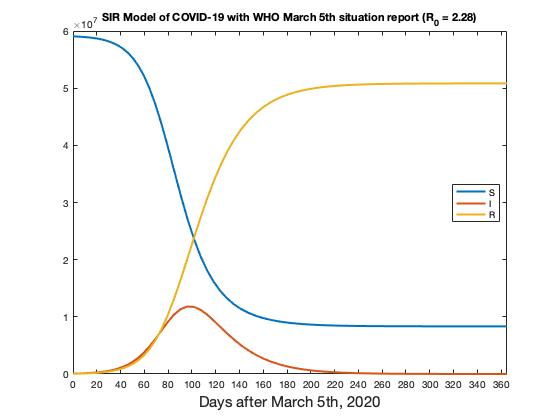
\includegraphics[scale=0.75]{plots/whosir228.jpg}
        
        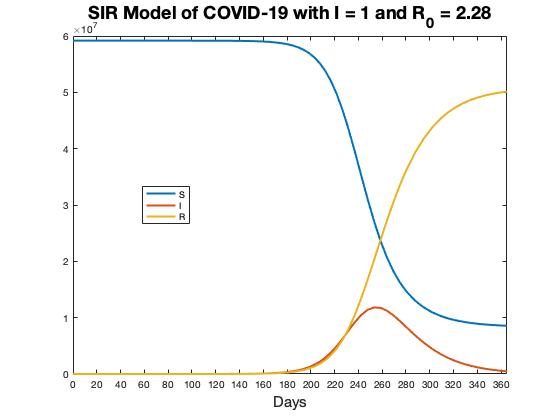
\includegraphics[scale=0.75]{plots/infect1_2.28.jpg}
        
        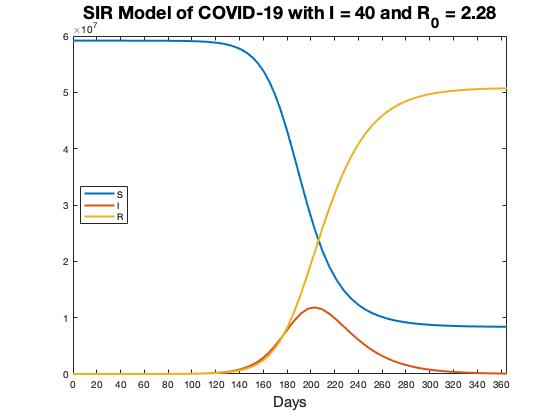
\includegraphics[scale=0.75]{plots/infect40_2.28.jpg}

        One thing that we can notice from these graphs is that there is not much difference in the shapes of the graphs based on the initial conditions. Our first model shows that the recovered population goes to approximately $5 \times 10^7$ individuals in the long term. Also, there is peak of around $1 \times 10^7$ infected individuals. These numbers do not change by very much across our trials. What we can notice is that there are different times of when the peaks will occur. The model based on WHO data has a peak occur at about 100 days, while the others have peaks at about 250 and 200 days. So, we can see that we can use our model as a basic indication of when to expect a large number of cases based on the initial conditions. This makes intuitive sense, as we would expect more cases to occur faster when starting with more infected individuals. Essentially, modifying the initial conditions determines when the peak of infections will happen.
        
        When we change the reproductive number, we can see that there are no major changes in the populations when $R_0$ is less than 1. It only becomes more serious when the number approaches 2. Using the estimated reproduction number, we can see that we can expect a large portion of the population to be infected at one time. This poses a serious threat to the population. What this model shows us is that it is necessary for preemptive measures to be taken to lower the reproductive number. If the reproductive number remains high, even with a small amount of infected individuals, it will spread through the majority of the population. Based on the simulations with a lower reproductive number, we believe that is very necessary to attempt to reduce this number. We can use our variations of the reproductive number using the WHO data as a forecast of what could occur. Given that this is currently the approximate amount of cases, we can see that we would expect very high amounts of cases given a constant reproductive number, again emphasizing the need to reduce it.
        
        More trials and graphs can be seen in the appendix section.
        
        \subsubsection{Equilibrium Analysis}
        
        We can apply equilibrium analysis techniques we have learned in class to our models. In order to solve for equilibrium points, we must set each partial derivative equal to zero. From the system of equations, we can see that this only occurs when the infected population is zero. In other words, $I(t)=0$ is the one condition we have for an equilibrium point. There is no restriction on what the populations for S and R are as long as we are still under the constraint that $N = S + R$. 
        
        In order to analyze the stability of the equilibria, we will take the partial derivative of each equation with respect to each variable. This method uses perturbations to see if the equilibria are stable or not. Thus, we have the matrix as follows:
        
        $$\begin{bmatrix}
            -\beta i & -\beta s & 0 \\
            \beta i & \beta s - \gamma & 0 \\
            0 & \gamma & 0 \\
        \end{bmatrix}$$
        
        In this matrix, the first row represents partials of $\frac{ds}{dt}$, the second row represents partials of $\frac{di}{dt}$, and the third row represents partials of $\frac{dr}{dt}$. The first column is with respect to s, the second column with respect to i, and the third column with respect to r. We can solve for the eigenvalues of this matrix by subtracting $\lambda I$ away from it and computing the determinant when it is equal to zero. This matrix is below:
        
        $$\begin{bmatrix}
            -\beta i-\lambda & -\beta s & 0 \\
            \beta i & \beta s - \gamma-\lambda & 0 \\
            0 & \gamma & -\lambda \\
        \end{bmatrix}$$
        
        We know that $\lambda$ represents the exponent of the solution to the perturbations, so a number less than or equal to zero represents a stable equilibrium if that is the case for all $\lambda$. If there is a single eigenvalue greater than or equal to zero, the equilibrium is unstable. We will end up with an equation of the form $-\lambda [(\beta s - \gamma - \lambda)(-\beta i - \lambda) + \beta^2si]=0$. We can see that we have a solution $\lambda_1=0$, and then solve when the interior is equal to zero.
        
        We can factor out terms and end with a quadratic equation of the form
        \newline $\lambda^2 + \lambda(\beta i - \beta s + \gamma) + \beta \gamma i  + \beta^2si = 0$. We know that in order for the equations to be equal to zero, we must have the condition that $i(t) = 0$. So, this will simplify to $\lambda^2 + \lambda(- \beta s + \gamma) = 0$. We can apply the quadratic formula to see that the solution below:
        \[
        \lambda_{2,3} = \frac{\beta s - \gamma \pm \sqrt{(\gamma - \beta s)^2}}{2} 
        \]   
        We can see that this solution will lead to $\lambda_2 = 0$ and $\lambda_3 = \beta s - \gamma$. We know that these coefficients must be less than or equal to zero for it to be a stable equilibrium point, and the determining factor is $\lambda_3$. We can see that the tipping point for this scenario is $\frac{\gamma}{\beta}$. If $s$ is greater than this number, then we have an unstable equilibrium point. This is because the exponent in the perturbation equation will be positive, which will make it increase infinitely over time. Thus, we must have a negative exponent so it will decay and so we won't depart from the equilibrium point. This is also known as the epidemic condition. If the initial starting amount of the susceptible population, then we are in a situation with epidemic conditions. If the starting $s$ is less than this, then we have a stable equilibrium and we are not in an epidemic scenario.
        
        To summarize, our equilibrium condition is: 
        \[
        \mbox{Unstable if: }s > \frac{\gamma}{\beta} \mbox{, stable if: }s \leq \frac{\gamma}{\beta}
        \]
        For example, we could have a solution of the form that $R(t)=N$ and $S(t)=0$ and $I(t)=0$. We can see that this intuitively makes sense as a stable point because there is no small change that will cause us to divert away from that equilibrium point. If a small number of people get infected, they will slowly move into the recovered compartment and thus we are back at our equilibrium point. If we have the opposite such that $S(t)=N$ and $R(t)=0$ and $I(t)=0$, we can see that a small increase in the amount of infected people can lead to a potentially huge outbreak as the infected population will grow. If we have a nonzero infected population, we can see that more individuals will get infected and more individuals will move to the recovered population, indicating we are not at an equilibrium point. So, our analysis aligns with what we would intuitively expect from our common knowledge of diseases.
        
        In our models, we took $\gamma$ as $1/18$ and $\beta$ as $0.126$ for our initial test. Thus, we can see that $\frac{\gamma}{\beta}$ is $0.439$. Therefore, we would not expect a stable equilibrium until the proportion of susceptible population falls below this level. This means that we are under epidemic conditions, and we can clearly see that there are large spikes in the population of infected individuals in our models because we are starting with the majority of the population in the susceptible compartment. Thus, we would expect that it is the case that we have a high number of infected and recovered individuals.
        
        We know that there are conditions for an epidemic using the reproductive number as well. This is the condition of when $R_0$ is greater than one. This implies that one person will infect more than one other person, so the disease will continue to spread. Our initial assumption indicates that we would be in an epidemic scenario, as we took $R_0$ as 2.28.
    
    \subsection{SEIR Model}
    
    We will attempt to make our model more rigorous by adding in an additional equation to our ODE system for the SEIR model. This adds more complexity to the basic compartmental model of SIR. While it is still not an accurate picture of what the spread of a virus is like in the real world, it represents a more realistic version than the SIR model.
    
    \subsubsection{Formulation}
    
    The SEIR model differs from the SIR model by adding in the compartment for the exposed population, in which that population has contracted the disease but is yet to reach an infectious state \cite{seir}. This is a more accurate representation of the real progression of a disease since there is an incubation period before an exposed individual can become infectious to other individuals. Parameters and variables are explained below:
        \begin{align*}
        S &= \text{ number of susceptible individuals}\\
        E &= \text{ number of exposed individuals}\\
        I &= \text{ number of infected individuals}\\
        R &= \text{ number of recovered individuals}\\
        N &= \text{ total population}\\
        \beta &= \text{ rate of exposure}\\
        \sigma &= \text{ rate of infection}\\
        \gamma &= \text{ rate of recovery}\\
        \end{align*}
        The system of differential equations thus becomes as follows:
        \begin{align*}
            \frac{dS}{dt} &= -\frac{\beta SI}{N} \\
            \frac{dE}{dt} &= \frac{\beta SI}{N} - \sigma E \\
            \frac{dI}{dt} &= \sigma E - \gamma I \\
            \frac{dR}{dt} &= \gamma I.
        \end{align*}
        And we have $S + E + I + R = N$.
        Thus, the total population is comprised of the total sum of each of the compartments of the population.
    
        These equations differ from our previous model by the inclusion of the exposed compartment. Now, there is a term of the exposed population in the infected equation, indicating individuals move from the exposed compartment to the infected compartment. The infected equation has the corresponding negative term. Other than these changes, these equations remain the same as in our previous model. We can modify these equations as we did in the last model as well by normalizing by N, and we get the following:
        \begin{align*}
            \frac{ds}{dt} &= -\beta si \\
            \frac{de}{dt} &= \beta si - \sigma e \\
            \frac{di}{dt} &= \sigma e - \gamma i \\
            \frac{dr}{dt} &= \gamma i.
        \end{align*}
        In this scenario, as previously, we can see that $s + e + i + r = 1$.

        We will undergo trials of this model using the same different initial condition scenarios as we previously did in the SIR model. We will also use the same variations in the reproductive number as well.
        
        Based on previously calculated and adjusted values in \cite{parameter}, we have set the rate of infection $\sigma=\frac{1}{5.2}$ since the mean incubation period of COVID-19 was calculated to be $5.2$ in an article by Li et al \cite{sigma}. In addition, we keep the rate of recovery $\gamma$ the same value we used in the SIR model. For the rate of exposure $\beta$, it follows the same ratio as the SIR model: 
        \[
            R_0 = \frac{\beta}{\gamma} \\
        \]
        $R_0$ is the reproductive number and $\gamma$ is the rate of recovery. Compared to the SIR model, we now have to consider the exposed population in our SEIR model. As proposed, we will set our initial exposed population $E$ as 20 times of the initial infected population $I$ \cite{parameter}. 
        
        \subsubsection{Results}
        
        The resulting graphs constructed using the SEIR model are below. We use the same trials of initial conditions as before.
        
        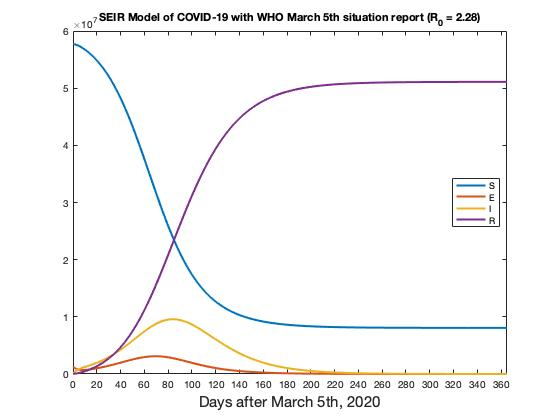
\includegraphics[scale=0.75]{plots/whoseir228.jpg}
        
        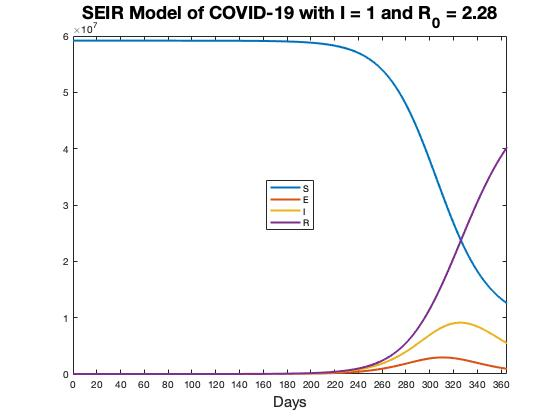
\includegraphics[scale=0.75]{plots/seir1r0.jpg}
        
        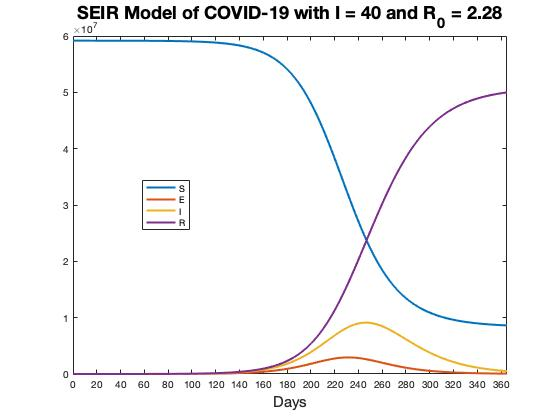
\includegraphics[scale=0.75]{plots/seir40r0.jpg}
        
       We can see now that there is much greater dependence on the initial conditions than in the previous model in terms of when the epidemic will happen. This is most apparent with the initial condition of one infected individual. We can see that the peak of infected and exposed individuals is lower than in the other graphs. We can also observe that the recovered population goes to about $4 \times 10^7$, while in the other graphs it goes to $5 \times 10^7$. We can see that the peak occurs later than in the other graphs. The peak with the WHO data occurs much sooner than in the other graphs, happening at about 90 days as opposed to 320 and 250 days. This has some implications. There are potentially more serious consequences that will come faster if there are higher initial conditions. This means that actively stopping a disease before it can spread to a significant amount of the population could potentially cause a much better response to the disease, as there will be more time to respond.
       
       % We know that this is important because the SEIR model is a more realistic representation of actual disease spread than the SIR model. This model places more emphasis on the initial conditions than the SIR model, which implies that it is necessary to proactively combat a disease as soon as possible. We can also draw similar conclusions based on the modification of the reproductive number. The results of these trials can be seen in the appendix.
        
        \subsubsection{Equilibrium Analysis}
        
        We can undergo a similar equilibrium analysis as in the last model. We can clearly see that the situation is the same as in the SIR model. In order for us to have an equilibrium point, we must have that $I(t)=0$ and that $E(t)=0$. This will make all equations go to zero. If we do not have these conditions met, we can clearly see that there will be some equations that are not equal to zero, and thus we will not be at an equilibrium point.
        
        In order to analyze the stability of the equilibria, we will take the partial derivative of each equation with respect to each variable. This method uses perturbations to see if the equilibria are stable or not. Thus, we have the matrix as follows below
        
        $$\begin{bmatrix}
            -\beta i & 0 & -\beta s & 0 \\
            \beta i & -\sigma & \beta s & 0 \\
            0 & \sigma & -\gamma & 0 \\
            0 & 0 & \gamma & 0 \\
        \end{bmatrix}$$.
        
        In this matrix, the first row represents partials of $\frac{ds}{dt}$, the second row represents partials of $\frac{de}{dt}$, the third row represents partials of $\frac{di}{dt}$, and the fourth row represents partials of $\frac{dr}{dt}$. The first column is with respect to s, the second column with respect to e, the third column with respect to i, and the fourth column with respect to r. We can solve for the eigenvalues of this matrix by subtracting $\lambda I$, taking the determinant, and setting it equal to zero. This matrix is below.
        
        $$\begin{bmatrix}
            -\beta i -\lambda & 0 & -\beta s & 0 \\
            \beta i & -\sigma -\lambda & \beta s & 0 \\
            0 & \sigma & -\gamma -\lambda & 0 \\
            0 & 0 & \gamma & -\lambda \\
        \end{bmatrix}$$
        
        We know that $\lambda$ represents the exponent of the solution to the perturbations, so a number less than or equal to zero represents a stable equilibrium if that is the case for all $\lambda$. If there is a single eigenvalue greater than or equal to zero, the equilibrium is unstable. When we do this computation, we see that we can solve using the equation:
        \[
        -\lambda [-\sigma[(-\beta i- \lambda)(\beta s) + (\beta i)(\beta s)]+(-\gamma-\lambda)[(-\beta i -\lambda)(-\sigma-\lambda)]]=0
        \]
        We can immediately see that $\lambda_1=0$ and can solve when the interior equals zero. By setting $i(t)=0$, our equilibrium condition, and combining terms, we can see that we get the following:
        \[
        -\lambda^3+\lambda^2(\gamma + \sigma)+\lambda(\sigma \beta s - \gamma \sigma)=0
        \]
        We can factor out a $-\lambda$ and see that $\lambda_2=0$ and are left with the following:
        \[
        -\lambda^2-\lambda(\gamma + \sigma)+(\sigma \beta s - \gamma \sigma)=0
        \]
        We can apply the quadratic formula to see that (allowing negatives to cancel):
        \[
        \lambda_{3,4}=\frac{-(\gamma + \sigma) \pm \sqrt{(\gamma + \sigma)^2 + 4(\sigma \beta s - \gamma\sigma)}}{2}
        \]
        
        If the susceptible population is greater than $\frac{\gamma}{\beta}$, then we know that we will have a positive $\lambda$, and thus equilibria of those conditions will be unstable. If we have that the susceptible population is below $\frac{\gamma}{\beta}$, then we know we will have negative $\lambda$ and that those equilibria will be stable points. We observe that this solution is the same as in the SIR model. We can summarize the stability below.
        \[
        \mbox{Unstable if: }s > \frac{\gamma}{\beta} \mbox{, stable if: }s \leq \frac{\gamma}{\beta}
        \]
        This will be our epidemic condition for this scenario as well. Intuitively, we would expect there to be a similar situation in terms of the stability as in the SIR model. All we have done is made the compartments more specific without changing any other aspects of the model. So, we would anticipate that the results for the requirements in the susceptible population to be the same.
        
        \subsection{SEIR Model With Vaccination}
        
        Because of its similarities to the common flu, it is not unrealistic to think that a vaccine could be made for COVID-19. We will consider the SEIR model and see what the benefits of having a vaccine are. This section will be prospective as a vaccine has yet to be developed.
        
        \subsubsection{Formulation}
        
        We have the same system as the SEIR model but under a few different conditions. Here, individuals can be immunized if they are in the susceptible population. We will consider the situation where a portion of the population gets vaccinated with each passing time period. In other words, when we use iterative methods, a portion of the susceptible population will move to the recovered, or immune, population each iteration. We get the following with these conditions:
        \begin{align*}
        S &= \text{ number of susceptible individuals}\\
        E &= \text{ number of exposed individuals}\\
        I &= \text{ number of infected individuals}\\
        R &= \text{ number of recovered individuals}\\
        N &= \text{ total population}\\
        \beta &= \text{ rate of exposure}\\
        \sigma &= \text{ rate of infection}\\
        \gamma &= \text{ rate of recovery}\\
        v &= \text{ rate of vaccination}\\
        \end{align*}
        Then, our system of differential equations becomes:
        \begin{align*}
            \frac{dS}{dt} &= \frac{\beta SI}{N} - vS \\
            \frac{dE}{dt} &= \frac{\beta SI}{N} - \sigma E \\
            \frac{dI}{dt} &= \sigma E - \gamma I \\
            \frac{dR}{dt} &= \gamma I + vS.
        \end{align*}
        And we have $S + E + I + R = N$. The only difference here is the rate of vaccination, $v$, which sends individuals directly from the susceptible compartment to the recovered compartment. All parameter values will be the same as in the previous models. Since the coronavirus comes from the same family as influenza, we will use statistics of the influenza vaccine to estimate the vaccination rate. The influenza vaccine is approximately 42 percent effective, averaged across age groups \cite{flu}. The rate of vaccination in China is estimated as 29.8 percent \cite{rate}. Again, China is known to not report statistics accurately, so we are using this as a tentative estimate. We multiply these together to get an approximate $v$ of $0.00034$, then by dividing by 365, to get an approximate rate for each period. We want to use this figure because our model is concerned with the portion of the population that will actually be moving to the recovered compartment; in other words, those that have been immunized. If we do the normalization by N, we get the following system:
        \begin{align*}
            \frac{ds}{dt} &= -\beta si - vs \\
            \frac{de}{dt} &= \beta si - \sigma e \\
            \frac{di}{dt} &= \sigma e - \gamma i \\
            \frac{dr}{dt} &= \gamma i + vs.
        \end{align*}
        We again see that $s + e + i + r = 1$. 
        
        We will undergo trials of this model using the same different initial condition scenarios as we previously did in the SIR and SEIR models. We will also use the same variations in the reproductive number as well.
        
        \subsubsection{Results}
        
        The graphs constructed using the vaccination system are below.
        
        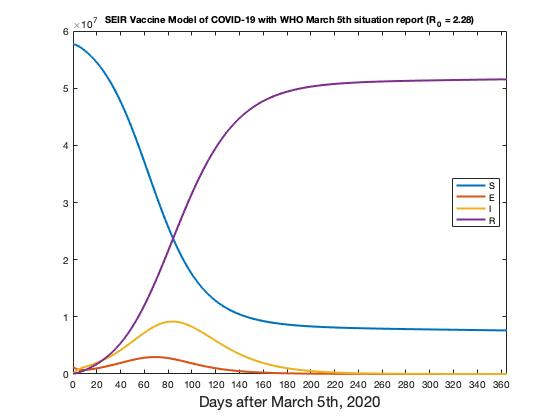
\includegraphics[scale=0.75]{plots/whoseirv228.jpg}
        
       The graph for initial condition of one infected individual starts with a higher time value in order to better capture the trend of the model.
        
        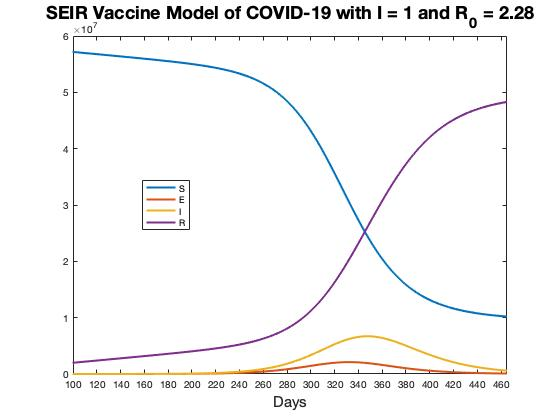
\includegraphics[scale=0.75]{plots/i1_seir_vac.jpg}
        
        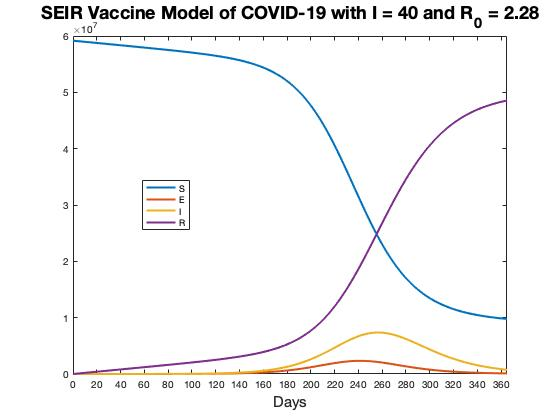
\includegraphics[scale=0.75]{plots/i40_seir_vac.jpg}
        
        We can see that the peak of infected individuals is lower, but still the major trends are the same as in the normal SEIR model. This implies that similar vaccination practices as influenza would not be enough on its own to combat the spread of the virus. There would either need to be a more effective vaccine than the influenza vaccine or much higher rates of vaccination in order to make a large portion of the population immune to the disease. This will be the case as long as the reproductive number is high. More trials and graphs can be seen in the appendix.
        
        \subsubsection{Equilibrium Analysis}
        
        We can undergo a similar equilibrium analysis as in the last model. We can clearly see that the situation is the same as in the SEIR model. In order for us to have an equilibrium point, we must have that $I(t)=0$ and that $E(t)=0$. This will make all equations go to zero. If we do not have these conditions met, we can clearly see that there will be some equations that are not equal to zero, and thus we will not be at an equilibrium point.
        
        In order to analyze the stability of the equilibria, we will take the partial derivative of each equation with respect to each variable. This method uses perturbations to see if the equilibria are stable or not. Thus, we have the matrix as follows below.
        
        $$\begin{bmatrix}
            -\beta i - v & 0 & -\beta s & 0 \\
            \beta i & -\sigma & \beta s & 0 \\
            0 & \sigma & -\gamma & 0 \\
            v & 0 & \gamma & 0 \\
        \end{bmatrix}$$
    
        In this matrix, the first row represents partials of $\frac{ds}{dt}$, the second row represents partials of $\frac{de}{dt}$, the third row represents partials of $\frac{di}{dt}$, and the fourth row represents partials of $\frac{dr}{dt}$. The first column is with respect to s, the second column with respect to e, the third column with respect to i, and the fourth column with respect to r. We can solve for the eigenvalues of this matrix by subtracting $\lambda I$, taking the determinant, and setting it equal to zero. This matrix is below.
        
        $$\begin{bmatrix}
            -\beta i - v -\lambda & 0 & -\beta s & 0 \\
            \beta i & -\sigma -\lambda & \beta s & 0 \\
            0 & \sigma & -\gamma -\lambda & 0 \\
            v & 0 & \gamma & -\lambda \\
        \end{bmatrix}$$
        
        We know that $\lambda$ represents the exponent of the solution to the perturbations, so a number less than or equal to zero represents a stable equilibrium if that is the case for all $\lambda$. If there is a single eigenvalue greater than or equal to zero, the equilibrium is unstable. When we do this computation, we see that we can solve using the equation:
        \[
        -\lambda [(-\gamma-\lambda)(-\sigma-\lambda)(-v-\lambda)-\sigma(\beta s)(-v-\lambda)]=0
        \]
        We can see $\lambda_1=0$ and work with the interior of the equation. We can factor out a term of $(-v-\lambda)$ to see that $\lambda_2=-v$ and are left with the following equation:
        \[
        (-v-\lambda)[(-\gamma-\lambda)(-\sigma-\lambda)-\beta\sigma s]=0
        \]
        Thus, we can solve for: 
        \[
        (-\gamma-\lambda)(-\sigma-\lambda)-\beta\sigma s=0
        \]
        Then, we can reduce to the following equation:
        \[
        \lambda^2+\lambda(\gamma+\sigma)+(\gamma \sigma-\beta \sigma s)=0
        \]
        We get the following with the quadratic formula:
        \[
        \lambda = \frac{-(\gamma+\sigma)\pm \sqrt{(\gamma+\sigma)^2-4(\gamma \sigma-\beta \sigma s)}}{2}
        \]
        So, we once again have the same solution of the following equilibrium conditions:
        \[
        \mbox{Unstable if: }s > \frac{\gamma}{\beta} \mbox{, stable if: }s \leq \frac{\gamma}{\beta}
        \]
        
        
        
    % \section{Results}
    
    % Things to consider: more graphs, discussions
    
    \section{Analysis}
    
    % Things to consider: epidemic scenarios, what situation is real world in, comparisons to real world (like a graph overlay of infected populations from model and the continued reported cases that is the real infected population)
    
    One thing that is interesting across all of our models is the same conditions for equilibrium. The equilibrium does not change even when vaccines are introduced into the population. We believe that this makes sense because the disease must be controlled to a certain extent. In other words, there must be a low enough population of susceptible individuals, regardless of what situation you are in.
    
    We can consider this level of the starting susceptible population as a critical level. In order to avoid a pandemic situation, the susceptible population must be below this level as our initial condition. We can investigate what happens if we alter the susceptible population to start below $\frac{\gamma}{\beta}$. We will move this population into the recovered population. We can consider this as a situation where a large portion of the population would be vaccinated or immune, and then see if the virus would spread from there. We can see this below.
    
    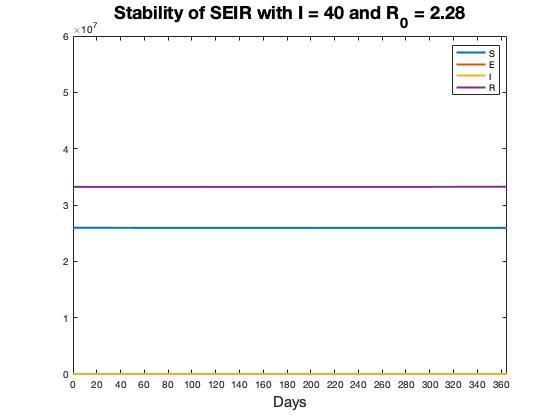
\includegraphics[scale=0.75]{plots/i40r228_st.jpg}
    
    We can see that the graphs stay very stable. We can see that the levels are not perfectly constant, and this is because we do not have a population of zero infected individuals. There are still some infected individuals, so we can see that there are very small changes. However, these are relatively insignificant. Furthermore, this implies that a large amount of the population needs to be vaccinated or immune in order to prevent an epidemic with a high enough reproductive number. This implies that a vaccine alone is not enough, as there will not be high enough levels of vaccination in any realistic situation. However, based on what we have seen, there is a critical population level that can be reached in order to stop the spread of the virus.
    
    Our models may not capture the true patterns of the spread of COVID-19. For instance, it is not certain whether recovered individuals stay immune to the disease after they have recovered. This means that our estimated number of recovered individuals may not remain as high as $5 \times 10^7$, so more information about the virus is needed in this regard in order to evaluate our model. There are additional models that cover this type of disease, such as the SIRS model. In this model, individuals in the recovered compartment will eventually move back into the susceptible compartment. An example of a disease that fits this is seasonal influenza.
    
    Additionally, our $R_0$ value is constant throughout a single simulation. This doesn't reflect reality, as $R_0$ could decrease as the response to fight the outbreak increases with more awareness of the disease. Some probable responses to prevent further spread of the disease are better sanitation techniques, quarantine of infected individuals, and restricting of movement of people. We have chosen to keep our reproductive number constant in order to gain a more basic understanding of the dynamics of the population compartments. However, all trials all emphasize the importance of attempting to reduce this number as the main way to prevent the spread of the virus.
    
    Across all our models with reproductive number $R_0$ greater than 2, we see that a very large portion of the population ends up in the recovered population. This shows that while majority of the population isn't infected at one given moment, most of the population will have contracted the disease. We can infer that there would be a devastating effect on businesses and productivity of the population if most of the people will get sick from this epidemic. This will also lead to more deaths. While COVID-19 has proven itself to be relatively safe to the majority of the population, increasing numbers of infected individuals will lead to more deaths overall. 
    
    Based on our results, we can see that if the reproductive number is high and people do not take action to reduce this constant, the disease will wreak havoc and it will spread through most of the population. As we have seen, there will not be a majority of people infected at once, but a large majority of people will come in contact with the virus at some point. This could prove very costly, as COVID-19 has shown itself to be a dangerous virus, causing 4,032 confirmed deaths at the time of writing \cite{who}.
    
    \section{Conclusions}
    
    After the completion of this paper, we believe we have made a successful attempt to model COVID-19. While there were areas where we could have made our model more rigorous and more complex, we completed and thoroughly investigated a simple base model for a serious and contemporary issue. We believe that our paper accurately represents a response that could be done when a public emergency like this happens. As our model gets more complex, it becomes more accurate. For those reasons, the SEIR model we completed was the best in the sense that it was the most realistic and would give the best picture if we were in a situation that required an accurate model. 
    
    Our models are not necessarily exactly the same as what is happening in the real world. As we have mentioned multiple times, it is possible to alter the reproductive number by taking proactive measures against the spread of the virus, such as social distancing and quarantines. Accordingly, we expect that in our model, with a constant reproductive number, that the spread of disease would be greater than in the real world. There are many other ways in which our model could be made more complex. The first is geographic scope. We have limited our investigation to the Hubei Province in China, the local epicenter of the outbreak. In order to create a more reasonable model, we could implement things such as travel across borders. This would allow us to investigate things such as travel bans, screening tests, and quarantines to investigate potential outcomes and how effective strategies could be against them. We could also make it more complex by integrating things such as self quarantine if you believe you have been exposed to the virus. This is relevant for people in our position, as we can learn from proactive strategies in China to see what is most effective here. We can see that potential travel and immigration strategy is relevant since the outbreak originated beyond our borders.
    
    Based on what we have presented here in our paper and what we are experiencing currently, we would expect the situation to continue to worsen in the United States. The amount of effort expended into combating the disease and the given state of infected individuals points to a continued expansion of the disease and large increases in the amount of infected people. There would need to be more proactive measures to stop the spread of the disease, in effect lowering the reproductive number, in order to prevent an epidemic situation in the United States. This is the case even when we have a vaccine, as that alone will not cause the prevention of the spread of the virus.
    
    As we have alluded to, epidemiological modeling is a necessary tool for us to employ. Disease does present a major threat to the well being of society, and tools such as this help us understand the nature of viruses like COVID-19 and the potential dangers that they possess to our collective health. Our model does address what we set out to do. It allows us to understand how to proceed from the beginning stages of dealing with a potential epidemic. In order to formulate a strategy on how to combat a viral outbreak, we must be able to understand what will happen. Our attempts to model COVID-19 do this in a way that is very basic but very necessary to try and contend with a phenomenon like this. As we have already stated, we have completed the first step any government or medical organization would do in order to develop a strategy to combat an epidemic, such as our estimation of a critical vaccination level. Our paper could not be entrenched in a more contemporaneous issue; as of March 11th, 2020 the World Health Organization has declared the outbreak to be a global pandemic. However, we are optimistic that more research can be done on COVID-19 to inform the scientific community and public to better prepare for the situations to come.
    
    % Big ideas, how does our model stack up, what makes the most sense, what is most accurate, what is most useful, what further could be done, how could it be more complex, more connections to real world, further applications
    \newpage
    
    \section{Appendix}
    
    For all models in the appendix, we also ran trials with $R_0$ as 0.9, but there were no discernible differences in our graphs to the 0.5 case. We also have not included graphs from our trials of starting with one infected individual because there were no differences visible in the shape of the graphs between those trials and the initial condition of 40. The only difference was the time frame of when infection peaks occurred. All graphs labeled with March $5^{th}$ situation report in the title use the WHO statistics as our initial condition. In addition, all graphs labeled with $I=40$ in the title starts with an initial condition of 40 infected individuals.

    \subsection{SIR Model Graphs}
    
   %  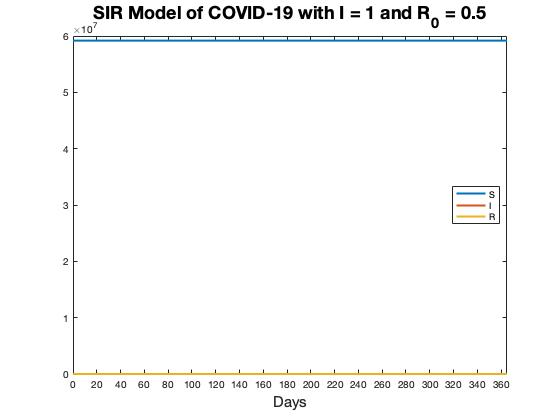
\includegraphics[scale=0.75]{plots/r0(0.5).jpg}
    
    % 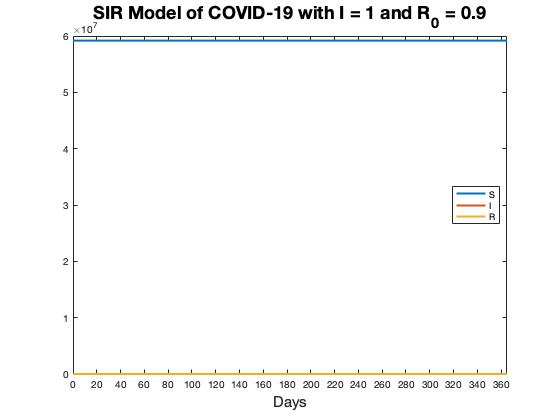
\includegraphics[scale=0.75]{plots/r0(0.9).jpg}
        
    % 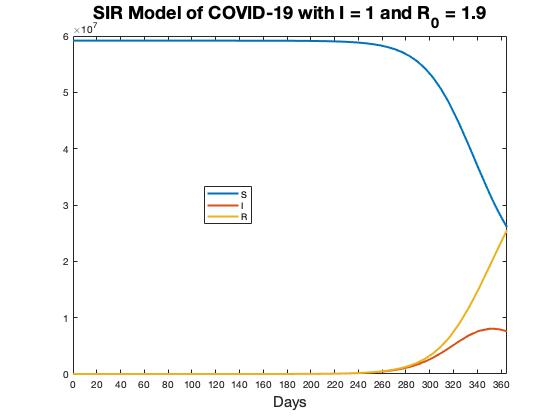
\includegraphics[scale=0.75]{plots/r0(1.9).jpg}
        
    % 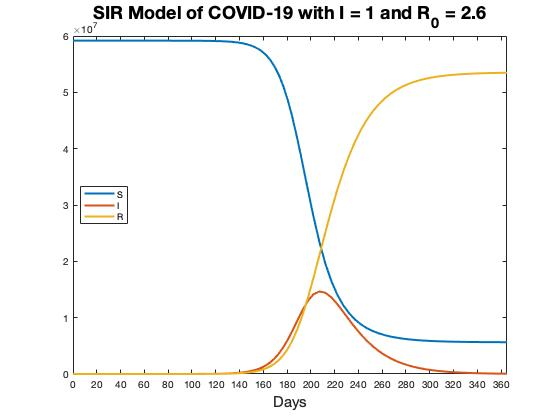
\includegraphics[scale=0.75]{plots/r0(2.6).jpg}
        
   %  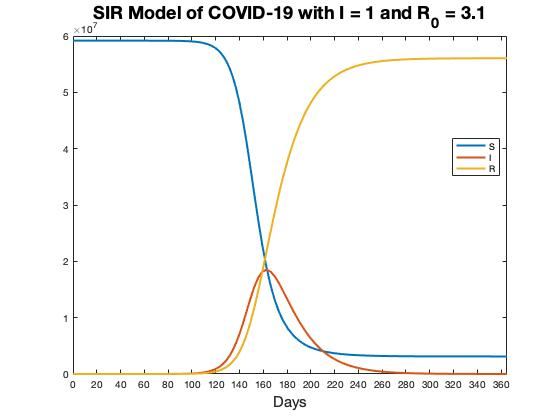
\includegraphics[scale=0.75]{plots/r0(3.1).jpg}
   
   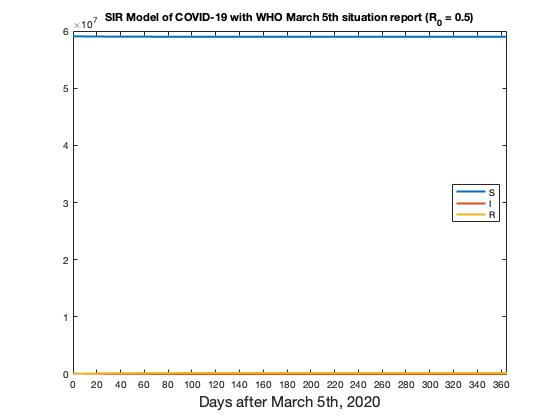
\includegraphics[scale=0.75]{plots/whosir5.jpg}
   
   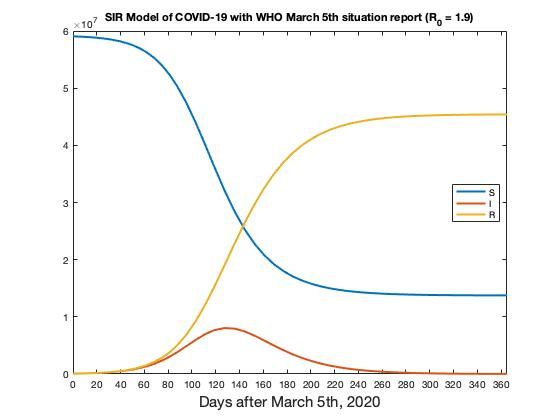
\includegraphics[scale=0.75]{plots/whosir19.jpg}
   
   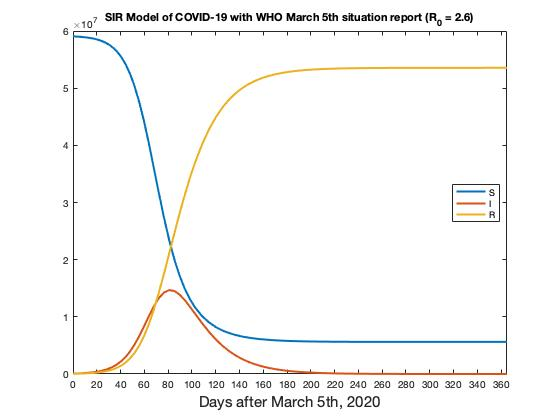
\includegraphics[scale=0.75]{plots/whosir26.jpg}
   
   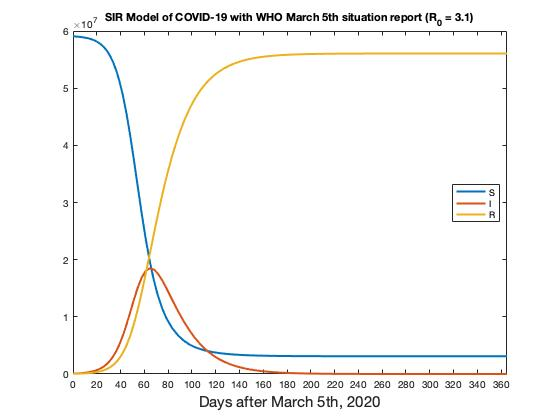
\includegraphics[scale=0.75]{plots/whosir31.jpg}
        
        
    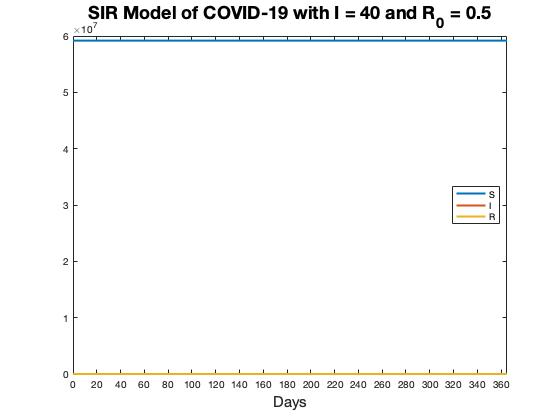
\includegraphics[scale=0.75]{plots/infect40(0.5).jpg}
        
    % 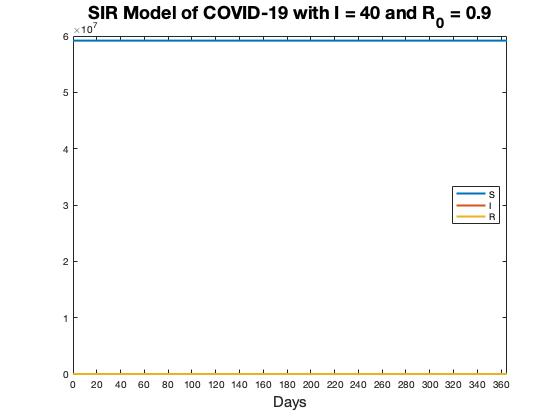
\includegraphics[scale=0.75]{plots/infect40(0.9).jpg}
        
    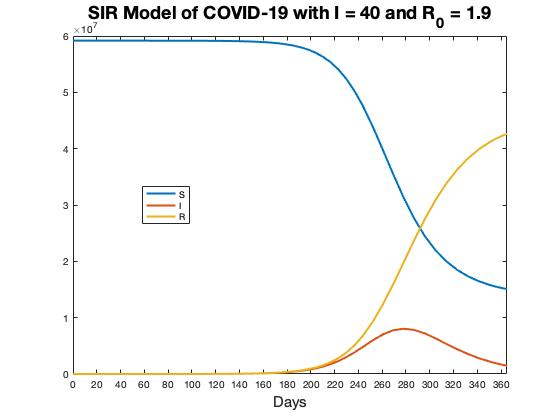
\includegraphics[scale=0.75]{plots/infect40(1.9).jpg}
        
    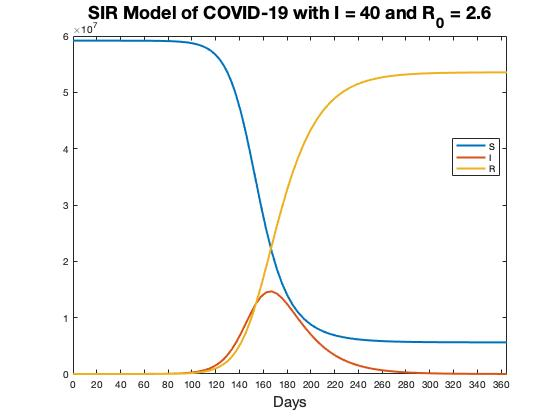
\includegraphics[scale=0.75]{plots/infect40(2.6).jpg}
        
    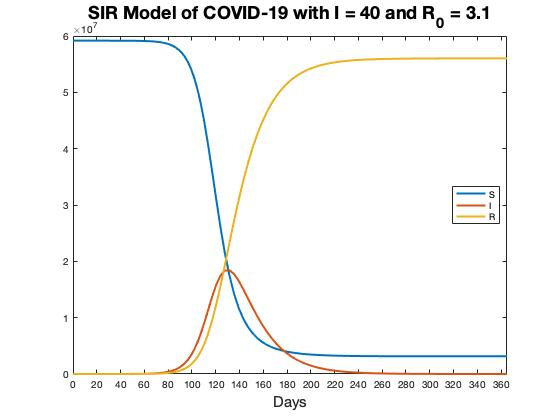
\includegraphics[scale=0.75]{plots/infect40(3.1).jpg}

    \subsection{SEIR Model Graphs}
    
    % Graphs for changing the reproductive number and initial condition of one infected individual are shown below.
    
    % 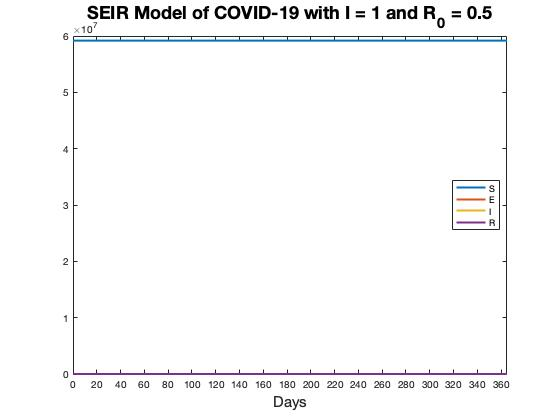
\includegraphics[scale=0.75]{plots/seir1(0.5).jpg}
        
    % 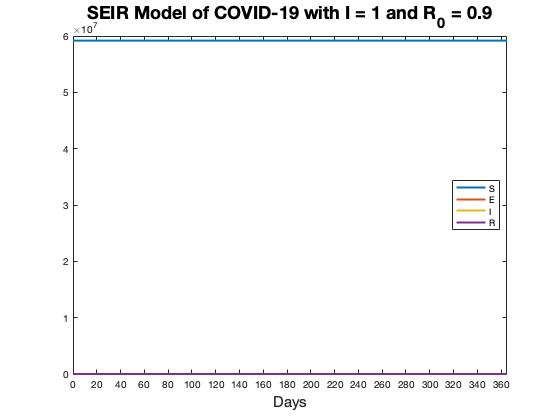
\includegraphics[scale=0.75]{plots/seir1(0.9).jpg}
        
    % 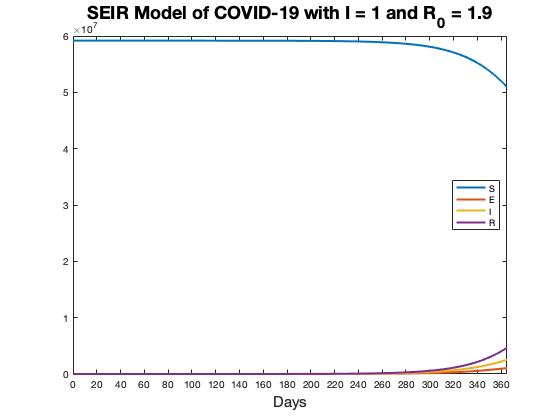
\includegraphics[scale=0.75]{plots/seir1(1.9).jpg}
        
    % 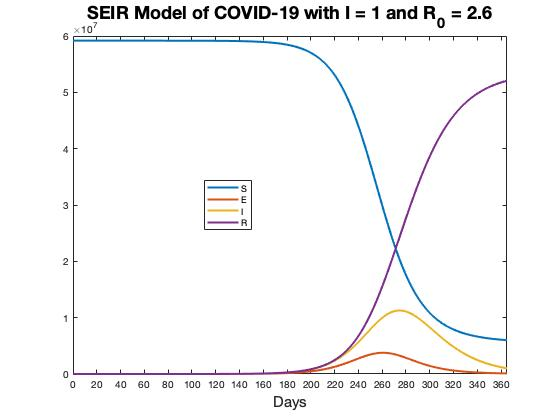
\includegraphics[scale=0.75]{plots/seir1(2.6).jpg}
        
    % 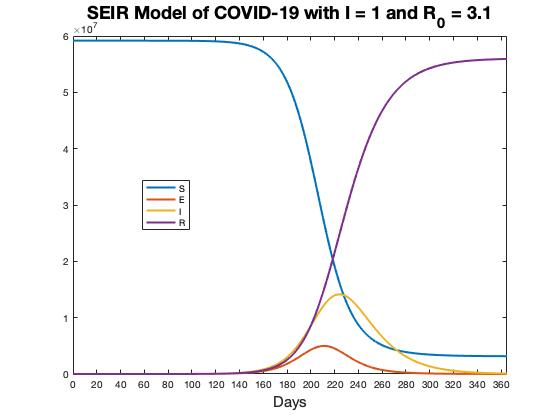
\includegraphics[scale=0.75]{plots/seir1(3.1).jpg}
            
    % Graphs for changing the reproductive number and initial condition of 40 infected individuals are shown below.
    
    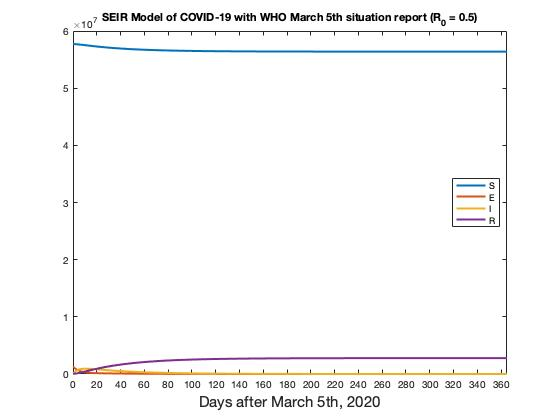
\includegraphics[scale=0.75]{plots/whoseir5.jpg}
    
    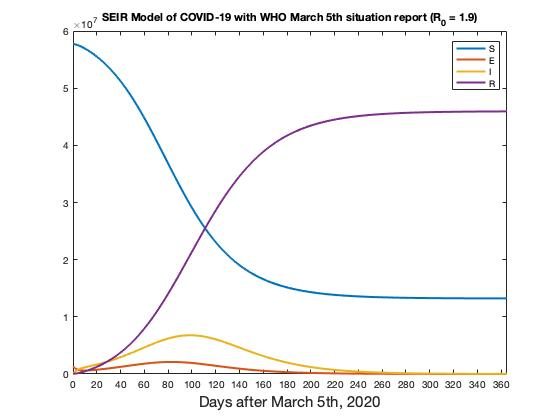
\includegraphics[scale=0.75]{plots/whoseir19.jpg}
    
    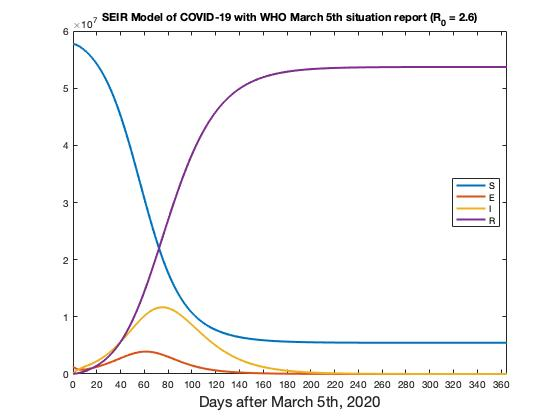
\includegraphics[scale=0.75]{plots/whoseir26.jpg}
    
    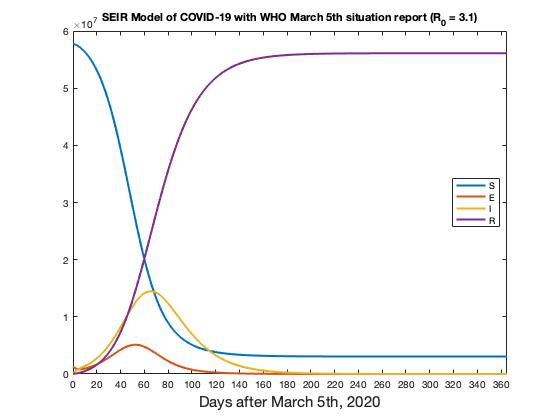
\includegraphics[scale=0.75]{plots/whoseir31.jpg}
        
    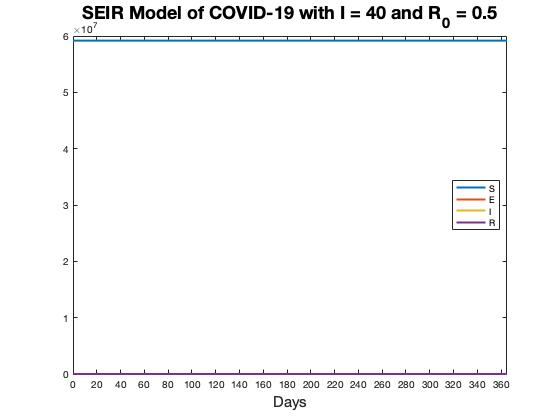
\includegraphics[scale=0.75]{plots/seir40(0.5).jpg}
        
    % 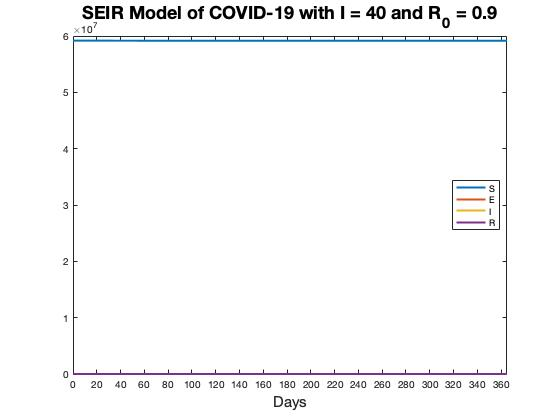
\includegraphics[scale=0.75]{plots/seir40(0.9).jpg}
        
    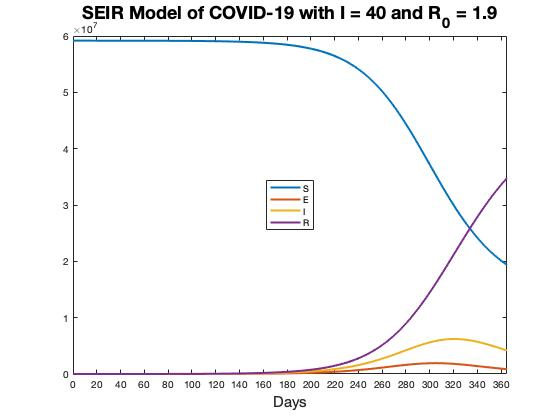
\includegraphics[scale=0.75]{plots/seir40(1.9).jpg}
        
    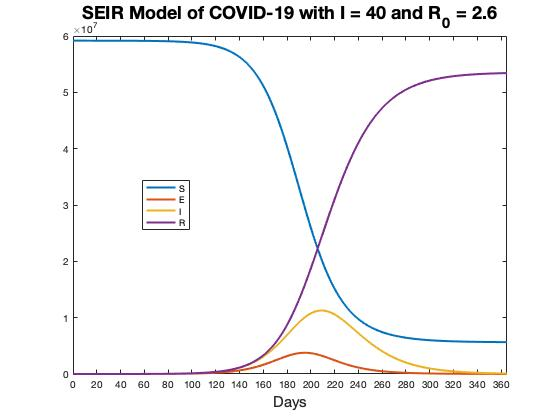
\includegraphics[scale=0.75]{plots/seir40(2.6).jpg}
        
    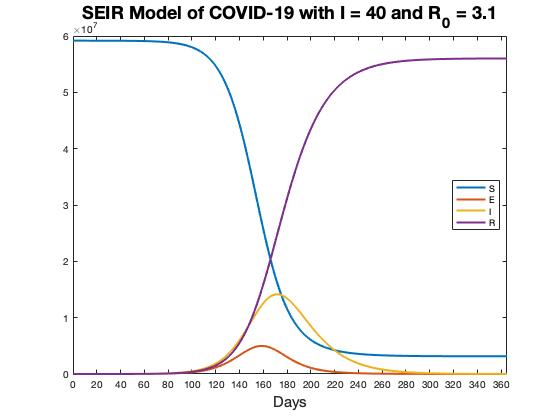
\includegraphics[scale=0.75]{plots/seir40(3.1).jpg}
    
    \subsection{SEIR Vaccine Model Graphs}
    
    % Graphs for changing the reproductive number and initial condition of one infected individual with vaccination available are shown below.

    % 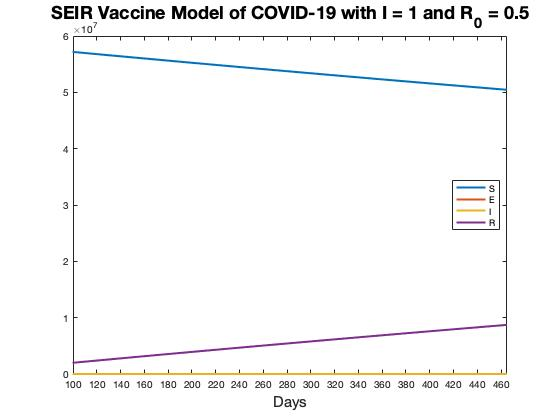
\includegraphics[scale=0.75]{plots/i1r5_seir_vac.jpg}
    
    % 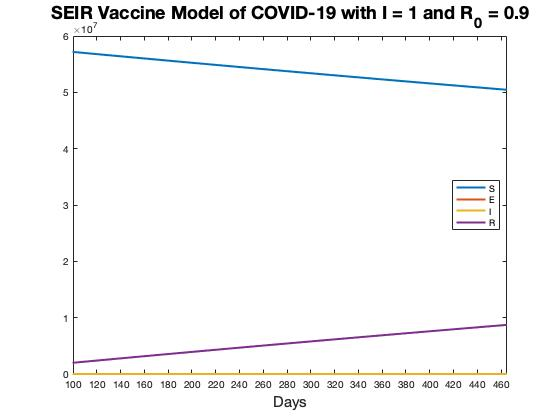
\includegraphics[scale=0.75]{plots/i1r9_seir_vac.jpg}
    
    % 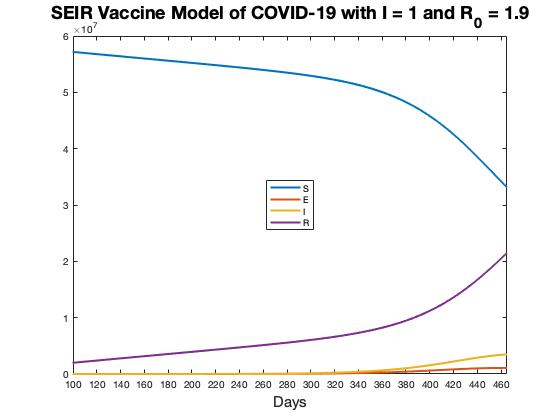
\includegraphics[scale=0.75]{plots/i1r19_seir_vac.jpg}
    
    % 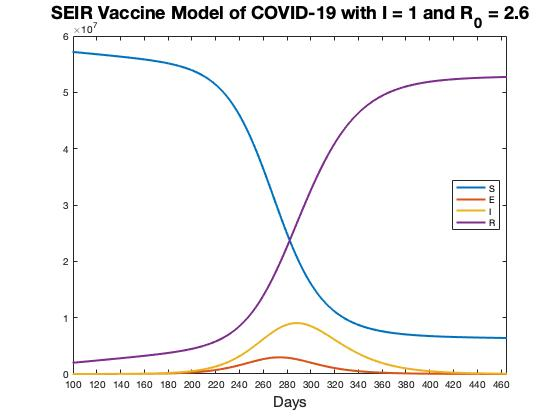
\includegraphics[scale=0.75]{plots/i1r26_seir_vac.jpg}
    
    % 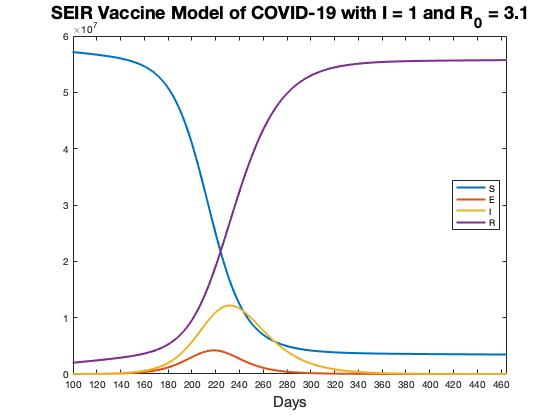
\includegraphics[scale=0.75]{plots/i1r31_seir_vac.jpg}
    
    % Graphs for changing the reproductive number and initial condition of 40 infected individuals with vaccination available are shown below.
    
    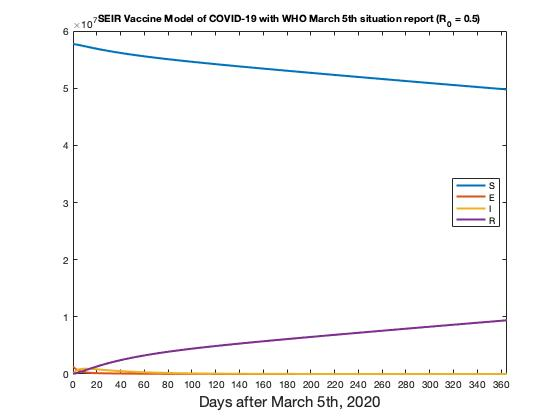
\includegraphics[scale=0.75]{plots/whoseirv5.jpg}
    
    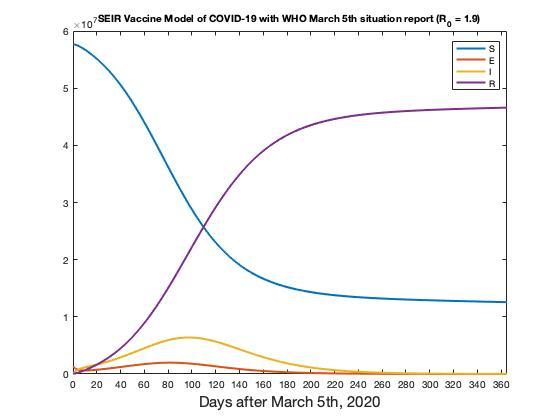
\includegraphics[scale=0.75]{plots/whoseirv19.jpg}
    
    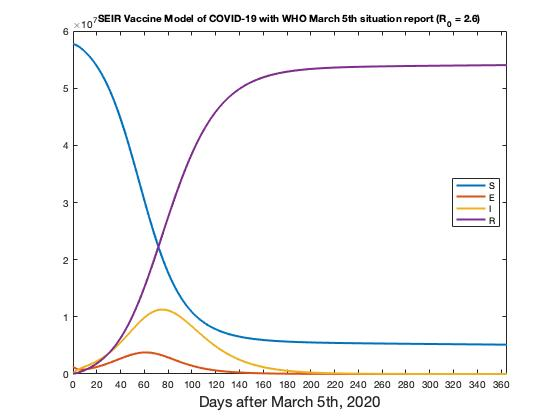
\includegraphics[scale=0.75]{plots/whoseirv26.jpg}
    
    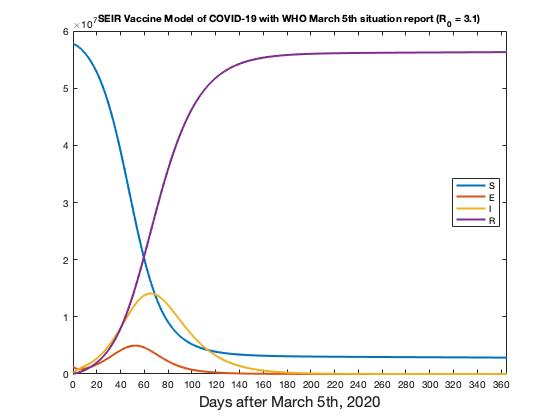
\includegraphics[scale=0.75]{plots/whoseirv31.jpg}
    
    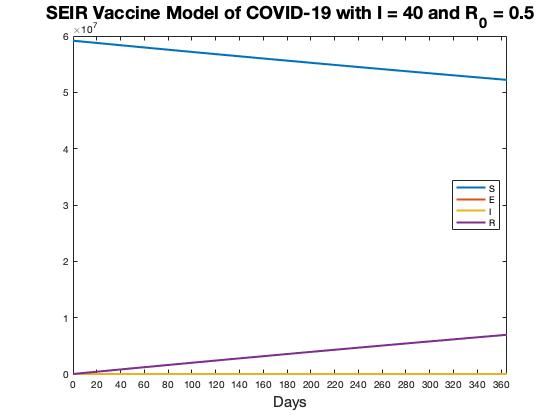
\includegraphics[scale=0.75]{plots/i40r5_seir_vac.jpg}
    
    % 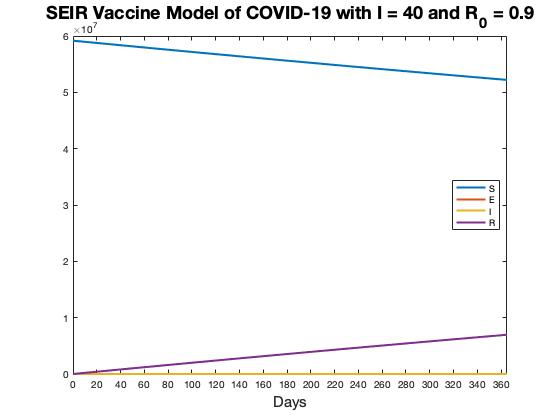
\includegraphics[scale=0.75]{plots/i40r9_seir_vac.jpg}
    
    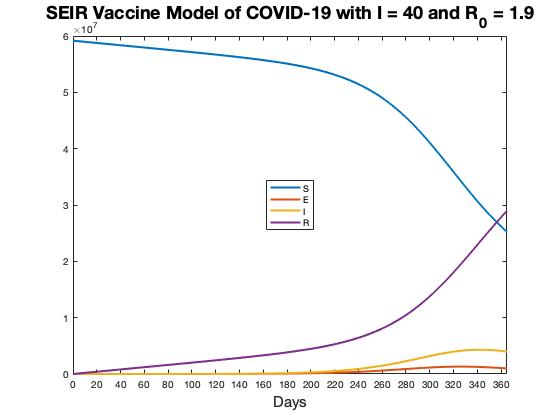
\includegraphics[scale=0.75]{plots/i40r19_seir_vac.jpg}
    
    \includegraphics[scale=0.75]{plots/i40r26_seir_vac.jpg}
 
    \includegraphics[scale=0.75]{plots/i40r31_seir_vac.jpg}
    
    \subsection{SEIR Stability Graphs}
    
    For these graphs, we start the initial level of the susceptible population below our epidemic condition of $\frac{\gamma}{\beta}$. We initialize $s(0)$ as this, where $\beta=R_0\gamma$. Refer back to the formulation of the SIR model in section 3.1.1 for more detailed explanation of these values.
    
    % Graphs for testing the susceptible population as a critical level are shown below. %may need to change
    
    % \includegraphics[scale=0.75]{plots/i40r5_st.jpg}
    
    % \includegraphics[scale=0.75]{plots/i40r9_st.jpg}
    
    \includegraphics[scale=0.75]{plots/i40r19_st.jpg}
    
    \includegraphics[scale=0.75]{plots/i40r26_st.jpg}
    
    \includegraphics[scale=0.75]{plots/i40r31_st.jpg}
    
    \newpage
    \subsection{MATLAB Code}
    
    \begin{lstlisting}
    % SIR Model function
    function dx = sir(t, x)
        dx = [0; 0; 0];
        r0 = 2.28; % Changed r0 to various other values
        gamma = 1/18; % recovery rate
        beta = r0*gamma; % infection rate
        dx(1) = -beta * x(1) * x(2);
        dx(2) = beta * x(1) * x(2) - gamma * x(2);
        dx(3) = gamma * x(2);
    end
    \end{lstlisting}
    
    \newpage
    
    \begin{lstlisting}
    % SIR model with WHO situation report data (S, I, and R values were changed to test I=1 and I=40 cases)
    N = 59170000; % population of Hubei Province
    I = 67466; % reported number of infected
    R = 40592; % reported number of recovered 
    S = N - I - R; % estimated number of susceptible 
    s = S/N; % the susceptible fraction of the population
    i = I/N; % the infected fraction of the population
    r = R/N; % the recovered fraction of the population
    props = [s i r];
    [t,x] = ode45('sir', [0 365], props);
    plot(t,N*x,'LineWidth',2);
    title('SIR Model of COVID-19 with WHO March 5th situation report','FontSize',12);
    xlabel('Days after March 5th, 2020','FontSize',15); 
    xlim([0 365]);
    xticks(0:20:365);
    ylim([0 60000000]);
    yticks(0:10000000:60000000);
    legend('S','I','R','Location','best');
    \end{lstlisting}
    
    \newpage
     
    \begin{lstlisting}
    % SEIR Model function
    function dx = seir(t, x)
        dx = [0; 0; 0; 0];
        r0 = 2.28; % Changed r0 to various other values
        gamma = 1/18; % recovery rate
        beta = r0*gamma; % exposure rate
        sigma = 1/(5.2); % infection rate
        dx(1) = -beta * x(1) * x(3);
        dx(2) = beta * x(1) * x(3) - sigma * x(2);
        dx(3) = sigma * x(2) - gamma * x(3);
        dx(4) = gamma * x(3);
    end
    \end{lstlisting}
    
    \begin{lstlisting}
    % SEIR Vaccine Model function
    function dx = seirv(t, x)
        dx = [0; 0; 0; 0];
        r0 = 2.28; % Changed r0 to various other values
        gamma = 1/18; % recovery rate
        beta = r0*gamma; % exposure rate
        sigma = 1/(5.2); % infection rate
        v = (.42*.298)/365; % vaccination rate
        dx(1) = (-beta * x(1) * x(3)) - (v * x(1));
        dx(2) = beta * x(1) * x(3) - (sigma * x(2));
        dx(3) = sigma * x(2) - gamma * x(3);
        dx(4) = (gamma * x(3)) + (v * x(1));
        end
    \end{lstlisting}
    
    \newpage
    
    \begin{lstlisting}
        % Testing stability of SEIR model 
        N = 59170000; % population of Hubei Province
        I = 40; % estimated intial number of infected
        E = 20*I; % estimated number of exposed
        R = 0; % number of recovered
        r0 = 2.28; % reproductive number (tested other r0 values)
        gamma = 1/18; % recovery rate
        beta = r0*gamma; % exposure rate
        s = gamma / beta; % the susceptible fraction of the population
        e = E/N; % the exposed fraction of the population
        i = I/N; % the infected fraction of the population
        r = 1 - e - i - (gamma / beta); % the recovered fraction of the population
        props = [s e i r];
        [t,x] = ode45('seir', [0 365], props);
        plot(t,N*x,'LineWidth',2);
        title('Stability of SEIR with I = 40 and R_0 = 2.28','FontSize',18);
        xlabel('Days','FontSize',15); 
        xlim([0 365]);
        xticks(0:20:365);
        ylim([0 60000000]);
        yticks(0:10000000:60000000);
        legend('S','E','I','R','Location','best');
    \end{lstlisting}
    
    \newpage
    
    \begin{lstlisting}
    % SEIR model with WHO situation report data (S, E, I, and R values were changed to test I=1 and I=40 cases)
    N = 59170000; % population of Hubei Province
    I = 67466; % reported number of infected
    E = 20*I; % estimated number of exposed
    R = 40592; % reported number of recovered
    S = N - I - R - E; % estimated number of susceptible 
    s = S/N; % the susceptible fraction of the population
    i = I/N; % the infected fraction of the population
    r = R/N; % the recovered fraction of the population
    e = E/N; % the exposed fraction of the population
    props = [s e i r];
    [t,x] = ode45('seir', [0 365], props);
    plot(t,N*x,'LineWidth',2);
    title('SEIR Model of COVID-19 with WHO March 5th situation report','FontSize',12);
    xlabel('Days after March 5th, 2020','FontSize',15); 
    xlim([0 365]);
    xticks(0:20:365);
    ylim([0 60000000]);
    yticks(0:10000000:60000000);
    legend('S','E','I','R','Location','best');
    \end{lstlisting}

\newpage
\printbibliography[heading=bibintoc,
title={7 References}
]


\end{document}